\section{Riemann Integration} 

  We would like to define an integral. We do this essentially by defining the Riemann sums for a particular partition, which is a number in $\mathbb{R}$. If we consider the set of all such Riemann sums, somehow bound them in a way. Then we define the upper and lower Riemann sums, and then consider the set of all Riemann sums. By doing so, we can construct two sets that are lower bounded and

  \begin{definition}[Partition]
    Let $[a, b]$ be an interval. A \textbf{partition} $P$ of $[a, b]$ is a set of $P = \{x_0, \ldots, x_n\}$ (note that this is finite!) s.t. 
    \begin{equation}
      a = x_0 \leq x_1 \leq \ldots \leq x_{n-1} \leq x_n = b
    \end{equation}
    with $\Delta x_i = x_i - x_{i-1}$ for $i = 1, \ldots, n$. 
  \end{definition}

  In some textbooks, we also define a \textit{partition with distinguished points} which simply is a partition $P$ along with some set of $\xi_i$'s that land in each interval. This allows for extra degrees of freedom for choosing points.  

  The natural way to define the Riemann integral is as the limit of the finite Riemann sums as partitions gets finer and finer.  But we must be careful in saying what ``finer'' means. It is not simply as the number of partitions $n \rightarrow \infty$, since this may lead to multiple subsequential values of convergence by increasing the partition within different subsets of $[a,b]$. 

  \begin{figure}[H]
    \centering
    % First row - upper sequence (red)
    \begin{subfigure}[b]{0.32\textwidth}
      \centering
      \begin{tikzpicture}[scale=0.8]
        % Axes
        \draw[->] (0,0) -- (4.5,0) node[right] {};
        \draw[->] (0,0) -- (0,3) node[above] {};
        
        % Origin label
        \node[below] at (0,0) {$0$};
        \node[below] at (4,0) {$4$};
        
        % Function curve
        \draw[thick] plot[domain=0:4, samples=100, smooth] coordinates {(0,0.6) (1,0.9) (2,1.5) (3,2.2) (4,2.8)};
        
        % Arrow at left end of curve
        \draw[->] (-0.2,0.6) -- (-0.4,0.6);
        % Arrow at right end of curve
        \draw[->] (3.8,2.7) -- (4.2,3.0);
        
        % Rectangles and patterns - rightmost is fixed
        \draw[red] (0,0) rectangle (1.33,0.9);
        \draw[red] (1.33,0) rectangle (2.67,1.5);
        \draw[red] (2.67,0) rectangle (4,2.8);
        
        % Fill with diagonal pattern
        \fill[pattern=north east lines, pattern color=red!40] (0,0) rectangle (1.33,0.9);
        \fill[pattern=north east lines, pattern color=red!40] (1.33,0) rectangle (2.67,1.5);
        \fill[pattern=north east lines, pattern color=red!40] (2.67,0) rectangle (4,2.8);
      \end{tikzpicture}
      \caption{}
    \end{subfigure}
    \hfill 
    \begin{subfigure}[b]{0.32\textwidth}
      \centering
      \begin{tikzpicture}[scale=0.8]
        % Axes
        \draw[->] (0,0) -- (4.5,0) node[right] {};
        \draw[->] (0,0) -- (0,3) node[above] {};
        
        % Origin label
        \node[below] at (0,0) {$0$};
        \node[below] at (4,0) {$4$};
        
        % Function curve
        \draw[thick] plot[domain=0:4, samples=100, smooth] coordinates {(0,0.6) (1,0.9) (2,1.5) (3,2.2) (4,2.8)};
        
        % Arrow at left end of curve
        \draw[->] (-0.2,0.6) -- (-0.4,0.6);
        % Arrow at right end of curve
        \draw[->] (3.8,2.7) -- (4.2,3.0);
        
        % Rectangles and patterns - rightmost is fixed
        \draw[red] (0,0) rectangle (0.67,0.7);
        \draw[red] (0.67,0) rectangle (1.33,0.9);
        \draw[red] (1.33,0) rectangle (2,1.3);
        \draw[red] (2,0) rectangle (2.67,1.7);
        \draw[red] (2.67,0) rectangle (4,2.8);
        
        % Fill with diagonal pattern
        \fill[pattern=north east lines, pattern color=red!40] (0,0) rectangle (0.67,0.7);
        \fill[pattern=north east lines, pattern color=red!40] (0.67,0) rectangle (1.33,0.9);
        \fill[pattern=north east lines, pattern color=red!40] (1.33,0) rectangle (2,1.3);
        \fill[pattern=north east lines, pattern color=red!40] (2,0) rectangle (2.67,1.7);
        \fill[pattern=north east lines, pattern color=red!40] (2.67,0) rectangle (4,2.8);
        
        % Red arrow showing refinement
        \draw[->, red, thick] (4.3,1.5) -- (4.8,1.5);
        \node[red] at (4.55,1.7) {$n\to\infty$};
      \end{tikzpicture}
      \caption{}
    \end{subfigure}
    \hfill 
    \begin{subfigure}[b]{0.32\textwidth}
      \centering
      \begin{tikzpicture}[scale=0.8]
        % Axes
        \draw[->] (0,0) -- (4.5,0) node[right] {};
        \draw[->] (0,0) -- (0,3) node[above] {};
        
        % Origin label
        \node[below] at (0,0) {$0$};
        \node[below] at (4,0) {$4$};
        
        % Function curve
        \draw[thick] plot[domain=0:4, samples=100, smooth] coordinates {(0,0.6) (1,0.9) (2,1.5) (3,2.2) (4,2.8)};
        
        % Arrow at left end of curve
        \draw[->] (-0.2,0.6) -- (-0.4,0.6);
        % Arrow at right end of curve
        \draw[->] (3.8,2.7) -- (4.2,3.0);
        
        % Rectangles and patterns - rightmost is fixed
        \draw[red] (0,0) rectangle (0.33,0.65);
        \draw[red] (0.33,0) rectangle (0.67,0.7);
        \draw[red] (0.67,0) rectangle (1,0.8);
        \draw[red] (1,0) rectangle (1.33,0.95);
        \draw[red] (1.33,0) rectangle (1.67,1.2);
        \draw[red] (1.67,0) rectangle (2,1.4);
        \draw[red] (2,0) rectangle (2.33,1.6);
        \draw[red] (2.33,0) rectangle (2.67,1.8);
        \draw[red] (2.67,0) rectangle (4,2.8);
        
        % Fill with diagonal pattern
        \fill[pattern=north east lines, pattern color=red!40] (0,0) rectangle (0.33,0.65);
        \fill[pattern=north east lines, pattern color=red!40] (0.33,0) rectangle (0.67,0.7);
        \fill[pattern=north east lines, pattern color=red!40] (0.67,0) rectangle (1,0.8);
        \fill[pattern=north east lines, pattern color=red!40] (1,0) rectangle (1.33,0.95);
        \fill[pattern=north east lines, pattern color=red!40] (1.33,0) rectangle (1.67,1.2);
        \fill[pattern=north east lines, pattern color=red!40] (1.67,0) rectangle (2,1.4);
        \fill[pattern=north east lines, pattern color=red!40] (2,0) rectangle (2.33,1.6);
        \fill[pattern=north east lines, pattern color=red!40] (2.33,0) rectangle (2.67,1.8);
        \fill[pattern=north east lines, pattern color=red!40] (2.67,0) rectangle (4,2.8);
        
        % Red arrow showing refinement with dots
        \draw[->, red, thick] (4.3,1.5) -- (4.8,1.5);
        \node[red] at (5.1,1.5) {$\cdots$};
      \end{tikzpicture}
      \caption{}
    \end{subfigure}
    
    % Second row - lower sequence (blue)
    \begin{subfigure}[b]{0.32\textwidth}
      \centering
      \begin{tikzpicture}[scale=0.8]
        % Axes
        \draw[->] (0,0) -- (4.5,0) node[right] {};
        \draw[->] (0,0) -- (0,3) node[above] {};
        
        % Origin label
        \node[below] at (0,0) {$0$};
        \node[below] at (4,0) {$4$};
        
        % Function curve
        \draw[thick] plot[domain=0:4, samples=100, smooth] coordinates {(0,0.6) (1,0.9) (2,1.5) (3,2.2) (4,2.8)};
        
        % Arrow at left end of curve
        \draw[->] (-0.2,0.6) -- (-0.4,0.6);
        % Arrow at right end of curve
        \draw[->] (3.8,2.7) -- (4.2,3.0);
        
        % Rectangles and patterns - leftmost is fixed
        \draw[blue] (0,0) rectangle (1.33,0.6);
        \draw[blue] (1.33,0) rectangle (2.67,1.2);
        \draw[blue] (2.67,0) rectangle (4,2.2);
        
        % Fill with diagonal pattern
        \fill[pattern=north east lines, pattern color=blue!40] (0,0) rectangle (1.33,0.6);
        \fill[pattern=north east lines, pattern color=blue!40] (1.33,0) rectangle (2.67,1.2);
        \fill[pattern=north east lines, pattern color=blue!40] (2.67,0) rectangle (4,2.2);
      \end{tikzpicture}
      \caption{}
    \end{subfigure}
    \hfill 
    \begin{subfigure}[b]{0.32\textwidth}
      \centering
      \begin{tikzpicture}[scale=0.8]
        % Axes
        \draw[->] (0,0) -- (4.5,0) node[right] {};
        \draw[->] (0,0) -- (0,3) node[above] {};
        
        % Origin label
        \node[below] at (0,0) {$0$};
        \node[below] at (4,0) {$4$};
        
        % Function curve
        \draw[thick] plot[domain=0:4, samples=100, smooth] coordinates {(0,0.6) (1,0.9) (2,1.5) (3,2.2) (4,2.8)};
        
        % Arrow at left end of curve
        \draw[->] (-0.2,0.6) -- (-0.4,0.6);
        % Arrow at right end of curve
        \draw[->] (3.8,2.7) -- (4.2,3.0);
        
        % Rectangles and patterns - leftmost is fixed
        \draw[blue] (0,0) rectangle (1.33,0.6);
        \draw[blue] (1.33,0) rectangle (2,1.2);
        \draw[blue] (2,0) rectangle (2.67,1.5);
        \draw[blue] (2.67,0) rectangle (3.33,2.0);
        \draw[blue] (3.33,0) rectangle (4,2.5);
        
        % Fill with diagonal pattern
        \fill[pattern=north east lines, pattern color=blue!40] (0,0) rectangle (1.33,0.6);
        \fill[pattern=north east lines, pattern color=blue!40] (1.33,0) rectangle (2,1.2);
        \fill[pattern=north east lines, pattern color=blue!40] (2,0) rectangle (2.67,1.5);
        \fill[pattern=north east lines, pattern color=blue!40] (2.67,0) rectangle (3.33,2.0);
        \fill[pattern=north east lines, pattern color=blue!40] (3.33,0) rectangle (4,2.5);
        
        % Blue arrow showing refinement
        \draw[->, blue, thick] (4.3,1.5) -- (4.8,1.5);
        \node[blue] at (4.55,1.7) {$n\to\infty$};
      \end{tikzpicture}
      \caption{}
    \end{subfigure}
    \hfill 
    \begin{subfigure}[b]{0.32\textwidth}
      \centering
      \begin{tikzpicture}[scale=0.8]
        % Axes
        \draw[->] (0,0) -- (4.5,0) node[right] {};
        \draw[->] (0,0) -- (0,3) node[above] {};
        
        % Origin label
        \node[below] at (0,0) {$0$};
        \node[below] at (4,0) {$4$};
        
        % Function curve
        \draw[thick] plot[domain=0:4, samples=100, smooth] coordinates {(0,0.6) (1,0.9) (2,1.5) (3,2.2) (4,2.8)};
        
        % Arrow at left end of curve
        \draw[->] (-0.2,0.6) -- (-0.4,0.6);
        % Arrow at right end of curve
        \draw[->] (3.8,2.7) -- (4.2,3.0);
        
        % Rectangles and patterns - leftmost is fixed
        \draw[blue] (0,0) rectangle (1.33,0.6);
        \draw[blue] (1.33,0) rectangle (1.67,1.1);
        \draw[blue] (1.67,0) rectangle (2,1.3);
        \draw[blue] (2,0) rectangle (2.33,1.5);
        \draw[blue] (2.33,0) rectangle (2.67,1.7);
        \draw[blue] (2.67,0) rectangle (3,1.9);
        \draw[blue] (3,0) rectangle (3.33,2.1);
        \draw[blue] (3.33,0) rectangle (3.67,2.3);
        \draw[blue] (3.67,0) rectangle (4,2.5);
        
        % Fill with diagonal pattern
        \fill[pattern=north east lines, pattern color=blue!40] (0,0) rectangle (1.33,0.6);
        \fill[pattern=north east lines, pattern color=blue!40] (1.33,0) rectangle (1.67,1.1);
        \fill[pattern=north east lines, pattern color=blue!40] (1.67,0) rectangle (2,1.3);
        \fill[pattern=north east lines, pattern color=blue!40] (2,0) rectangle (2.33,1.5);
        \fill[pattern=north east lines, pattern color=blue!40] (2.33,0) rectangle (2.67,1.7);
        \fill[pattern=north east lines, pattern color=blue!40] (2.67,0) rectangle (3,1.9);
        \fill[pattern=north east lines, pattern color=blue!40] (3,0) rectangle (3.33,2.1);
        \fill[pattern=north east lines, pattern color=blue!40] (3.33,0) rectangle (3.67,2.3);
        \fill[pattern=north east lines, pattern color=blue!40] (3.67,0) rectangle (4,2.5);
        
        % Blue arrow showing refinement with dots
        \draw[->, blue, thick] (4.3,1.5) -- (4.8,1.5);
        \node[blue] at (5.1,1.5) {$\cdots$};
      \end{tikzpicture}
      \caption{}
    \end{subfigure}
    
    \caption{Upper (top row) and lower (bottom row) Riemann sums with refinement of partition. In the upper row, the rightmost rectangle remains fixed while other rectangles become thinner. In the lower row, the leftmost rectangle remains fixed while other rectangles become thinner.}
    \label{fig:upper-lower-refinement}
  \end{figure}

  An alternative way is to have the partitions all converge ``uniformly'' as in the maximum length of an interval in a partition must go to $0$. 

  \begin{figure}[H]
    \centering
    \begin{subfigure}[b]{0.32\textwidth}
      \centering
      \begin{tikzpicture}[scale=0.9]
        % Axes
        \draw[->] (0,0) -- (4.5,0) node[right] {};
        \draw[->] (0,0) -- (0,3) node[above] {};
        
        % Origin label
        \node[below] at (0,0) {$0$};
        \node[below] at (4,0) {$4$};
        
        % Rectangles and patterns
        \draw[blue] (0,0) rectangle (2,1.2);
        \draw[blue] (2,0) rectangle (4,2.2);
        
        % Fill with diagonal pattern
        \fill[pattern=north east lines, pattern color=blue!40] (0,0) rectangle (2,1.2);
        \fill[pattern=north east lines, pattern color=blue!40] (2,0) rectangle (4,2.2);
        
        % Function curve
        \draw[thick] plot[domain=0:4, samples=100, smooth] coordinates {(0,0.6) (1.5,1.2) (2.5,1.8) (4,2.8)};
        
        % Label f (no arrow)
        \node at (4.2,2.6) {$f$};
      \end{tikzpicture}
      \caption{$\lambda(P) = 2$}
    \end{subfigure}
    \hfill 
    \begin{subfigure}[b]{0.32\textwidth}
      \centering
      \begin{tikzpicture}[scale=0.9]
        % Axes
        \draw[->] (0,0) -- (4.5,0) node[right] {};
        \draw[->] (0,0) -- (0,3) node[above] {};
        
        % Origin label
        \node[below] at (0,0) {$0$};
        \node[below] at (4,0) {$4$};
        
        % Rectangles and patterns
        \draw[blue] (0,0) rectangle (1,0.8);
        \draw[blue] (1,0) rectangle (2,1.5);
        \draw[blue] (2,0) rectangle (3,2);
        \draw[blue] (3,0) rectangle (4,2.5);
        
        % Fill with diagonal pattern
        \fill[pattern=north east lines, pattern color=blue!40] (0,0) rectangle (1,0.8);
        \fill[pattern=north east lines, pattern color=blue!40] (1,0) rectangle (2,1.5);
        \fill[pattern=north east lines, pattern color=blue!40] (2,0) rectangle (3,2);
        \fill[pattern=north east lines, pattern color=blue!40] (3,0) rectangle (4,2.5);
        
        % Function curve
        \draw[thick] plot[domain=0:4, samples=100, smooth] coordinates {(0,0.6) (1.5,1.2) (2.5,1.8) (4,2.8)};
        
        % Label f (no arrow)
        \node at (4.2,2.6) {$f$};
      \end{tikzpicture}
      \caption{$\lambda(P) = 1$}
    \end{subfigure}
    \hfill 
    \begin{subfigure}[b]{0.32\textwidth}
      \centering
      \begin{tikzpicture}[scale=0.9]
        % Axes
        \draw[->] (0,0) -- (4.5,0) node[right] {};
        \draw[->] (0,0) -- (0,3) node[above] {};
        
        % Origin label
        \node[below] at (0,0) {$0$};
        \node[below] at (4,0) {$4$};
        
        % Rectangles and patterns
        \draw[blue] (0,0) rectangle (0.5,0.7);
        \draw[blue] (0.5,0) rectangle (1,0.9);
        \draw[blue] (1,0) rectangle (1.5,1.1);
        \draw[blue] (1.5,0) rectangle (2,1.4);
        \draw[blue] (2,0) rectangle (2.5,1.7);
        \draw[blue] (2.5,0) rectangle (3,2);
        \draw[blue] (3,0) rectangle (3.5,2.3);
        \draw[blue] (3.5,0) rectangle (4,2.6);
        
        % Fill with diagonal pattern
        \fill[pattern=north east lines, pattern color=blue!40] (0,0) rectangle (0.5,0.7);
        \fill[pattern=north east lines, pattern color=blue!40] (0.5,0) rectangle (1,0.9);
        \fill[pattern=north east lines, pattern color=blue!40] (1,0) rectangle (1.5,1.1);
        \fill[pattern=north east lines, pattern color=blue!40] (1.5,0) rectangle (2,1.4);
        \fill[pattern=north east lines, pattern color=blue!40] (2,0) rectangle (2.5,1.7);
        \fill[pattern=north east lines, pattern color=blue!40] (2.5,0) rectangle (3,2);
        \fill[pattern=north east lines, pattern color=blue!40] (3,0) rectangle (3.5,2.3);
        \fill[pattern=north east lines, pattern color=blue!40] (3.5,0) rectangle (4,2.6);
        
        % Function curve
        \draw[thick] plot[domain=0:4, samples=100, smooth] coordinates {(0,0.6) (1.5,1.2) (2.5,1.8) (4,2.8)};
        
        % Label f (no arrow)
        \node at (4.2,2.6) {$f$};
      \end{tikzpicture}
      \caption{$\lambda(P) = 0.5$}
    \end{subfigure}
    \caption{Approximating an integral with increasingly fine partitions}
    \label{fig:partition-refinement}
  \end{figure}

  A cleaner way it to simply look at the set of all partitions along with the set of the corresponding upper and lower Riemann sums, and then hope that they behave nicely with each other. This is the approach we will take. 

  \begin{definition}[Riemann Sums with Respect to Partition]
    Let $P$ be a partition of $[a, b]$ and $f: [a, b] \to \mathbb{R}$ be bounded. Then, the \textbf{upper and lower Riemann sum} is defined 
    \begin{equation}
      M_i = \sup_{\Delta x_i} f(x), \qquad m_i = \inf_{\Delta x_i} f(x) 
    \end{equation}
    Now define  
    \begin{equation}
      U(P, f) = \sum_{i=1}^n M_i \Delta x_i, \qquad L(P, f) = \sum_{i=1}^n m_i \Delta x_i
    \end{equation}

    \begin{figure}[H]
      \centering 
      \begin{tikzpicture}[scale=0.9]
        % Define axes
        \draw[->] (-0.5,0) -- (10.5,0) node[right] {$x$};
        \draw[->] (0,-0.5) -- (0,5) node[above] {$y$};
        
        % Function curve
        \draw[thick] plot[domain=0:10, samples=100, smooth] 
            coordinates {(0,2.5) (2,1.8) (4,1.5) (6,2) (8,3.2) (10,4.5)};
        
        % f label
        \node at (10.5,4.5) {$f$};
        
        % Partition points on x-axis
        \foreach \x/\label [count=\i from 0] in {
          0/a=x_0, 2/x_1, 4/x_2, 6/x_3, 8/x_4, 10/b=x_5
        } {
          \fill (\x,0) circle (0.07);
          \node[black, below, font=\footnotesize] at (\x,-0.35) {$\label$};
        }
        
        % Sample points ξᵢ (blue)
        \foreach \x/\label [count=\i from 1] in {
          1.1/\xi_1, 2.5/\xi_2, 5.4/\xi_3, 7.7/\xi_4, 9.5/\xi_5
        } {
          \fill[blue] (\x,0) circle (0.05);
          \node[blue, below, font=\footnotesize] at (\x,0) {$\label$};
          
        }
        \draw[blue, thin] (1.1,0) -- (1.1,2.1);
        \draw[blue, thin] (2.5,0) -- (2.5,1.7);
        \draw[blue, thin] (5.4,0) -- (5.4,1.8);
        \draw[blue, thin] (7.7,0) -- (7.7,3);
        \draw[blue, thin] (9.5,0) -- (9.5,4.2);
        
        % Rectangles for Riemann sum
        \foreach \xstart/\xend/\y [count=\i from 1] in {
          0/2/2.1, 2/4/1.7, 4/6/1.8, 6/8/3, 8/10/4.2
        } {
          % Rectangle with red border and pattern
          \draw[red] (\xstart,0) rectangle (\xend,\y);
          \fill[pattern=north east lines, pattern color=red!40] (\xstart,0) rectangle (\xend,\y);
          
          % Function value labels
          \node[red] at ({(\xstart+\xend)/2},{\y+0.3}) {$f(\xi_{\i})$};
        }
        
        % Delta x labels with curly braces (opening downward)
        \foreach \xstart/\xend/\i in {
          0/2/1, 2/4/2, 4/6/3, 6/8/4, 8/10/5
        } {
          \draw[decorate, decoration={brace, mirror, amplitude=8pt}, black] 
            (\xstart,-0.8) -- (\xend,-0.8) node[midway, below, yshift=-6pt] {$\Delta x_{\i}$};
        }
      \end{tikzpicture}
      \caption{Riemann sum approximation using sample points $\xi_i$ within each subinterval. This is known as a Riemann sum of a partition with distinguished points. The Riemann sum is a mapping that takes in a partition with distinguished points $p = (P, \xi)$ on the closed interval $[a, b]$ and outputs a number representing the total area of the Riemann sums. }
      \label{fig:riemann-sum-xi}
    \end{figure}
  \end{definition}

  \begin{definition}[Riemann Integral]
    Now, given the same assumptions, the \textbf{upper and lower Rimemann integrals} of $f(x)$ are defined 
    \begin{equation}
      \int_a^{\bar{b}} f(x) \, dx \coloneqq \inf_P U(P, f), \qquad \int_{\bar{a}}^{b} f(x) \, dx \coloneqq \sup_P L(P, f)
    \end{equation}
    If the upper and lower Riemann integrals are equal, then $f$ is said to be \textbf{Riemann integrable} over $[a, b]$, denoted $f \in \mathcal{R}([a, b])$.\footnote{Where $\mathcal{R}(X)$ is the set of all Riemann integrable functions over $X$.}
  \end{definition} 

  Great, so we've defined Riemann integrable functions, but it's hard to determine whether a function is Riemann integrable---and if so---what the value of the integral is. We will determine the first problem by talking about sufficient conditions for Riemann integrability, and then introduce the fundamental theorem of calculus to address computability. 

  \begin{definition}[Refinement]
    $P^\ast$ is a \textbf{refinement} of $P$ if $P \subset P^\ast$. If $P_1, P_2$ are two partitions, then their \textbf{common refinement} $P^\ast = P_1 \cup P_2$. 

    \begin{figure}[H]
      \centering 
      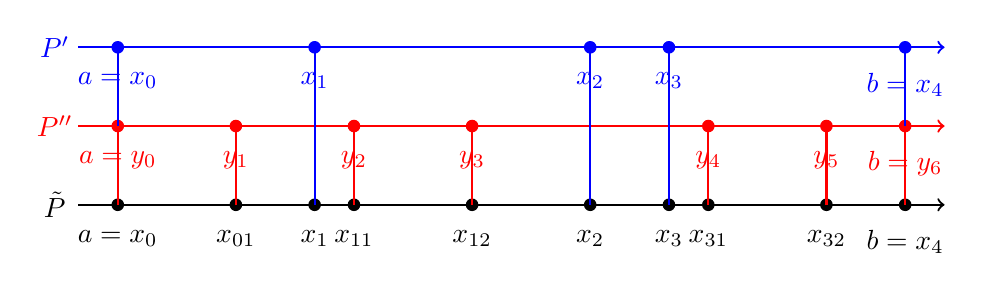
\begin{tikzpicture}[scale=1.0]
        % First partition P' (blue) - reduced vertical spacing
        \draw[thick, blue, ->] (-0.5,1) -- (10.5,1);
        \node[blue] at (-0.8,1) {$P'$};
        
        % Points on first partition
        \foreach \x/\label [count=\i from 0] in {
          0/a=x_0, 2.5/x_1, 6/x_2, 7/x_3, 10/b=x_4
        } {
          \fill[blue] (\x,1) circle (0.08);
          \node[blue, below] at (\x,0.8) {$\label$};
        }
        
        % Second partition P'' (red) - reduced vertical spacing
        \draw[thick, red, ->] (-0.5,0) -- (10.5,0);
        \node[red] at (-0.8,0) {$P''$};
        
        % Points on second partition
        \foreach \x/\label [count=\i from 0] in {
          0/a=y_0, 1.5/y_1, 3/y_2, 4.5/y_3, 7.5/y_4, 9/y_5, 10/b=y_6
        } {
          \fill[red] (\x,0) circle (0.08);
          \node[red, below] at (\x,-0.2) {$\label$};
        }
        
        % Third partition P̃ (black) - combined partition - reduced vertical spacing
        \draw[thick, ->] (-0.5,-1) -- (10.5,-1);
        \node at (-0.8,-1) {$\tilde{P}$};
        
        % Points on combined partition - all points from both partitions
        \foreach \x/\label [count=\i from 0] in {
          0/a=x_0, 1.5/x_{01}, 2.5/x_1, 3/x_{11}, 4.5/x_{12}, 6/x_2, 7/x_3, 7.5/x_{31}, 9/x_{32}, 10/b=x_4
        } {
          \fill (\x,-1) circle (0.08);
          \node[below] at (\x,-1.2) {$\label$};
        }
        
        % Vertical lines connecting corresponding points
        % From P' to P̃
        \foreach \x in {0, 2.5, 6, 7, 10} {
          \draw[blue, thick] (\x,1) -- (\x,-1);
        }
        
        % From P'' to P̃
        \foreach \x in {0, 1.5, 3, 4.5, 7.5, 9, 10} {
          \draw[red, thick] (\x,0) -- (\x,-1);
        }
      \end{tikzpicture}
      \caption{Partitions $P'$ and $P''$ with their common refinement $\tilde{P}$}
      \label{fig:three-partitions}
    \end{figure}
  \end{definition}

  \begin{lemma}[Fundamental Lemma]
    If $P^\ast$ is a refinement of $P$ and $f: [a, b] \to \mathbb{R}$ is bounded, then 
    \begin{equation}
      L(P, f) \leq L(P^\ast, F) \leq U(P^\ast, F) \leq U(P, f) 
    \end{equation}
  \end{lemma}
  \begin{proof} 
    By induction on the number of points we add to $P$ to get $P^\ast$, we might as well assume that $P^\ast = P \cup \{x_\ast\}$. So, 
    \begin{align}
      P & = \{a = x_0, x_1, \ldots, x_{n-1}, x_n \} \\
      P^\ast & = \{a = x_0, x_1, \ldots, x_{i-1}, x_i, x_\ast, x_{i+1}, \ldots, x_{n-1}, x_n \} \\
    \end{align}
    Now let's compute $L(f, P^\ast) - L(f, P)$. Since the only intervals affected are $[x_i, x_{i+1}]$, we have 
    \begin{align}
      L(f, P^\ast) - L(f, P) & = \inf_{[x_i, x_{\ast}]} f(x) (x_{\ast} - x_i) + \inf_{[x_\ast, x_{i+1}]} f(x) (x_{i+1} - x_\ast) - \inf_{[x_{i}, x_{i+1}]} f(x) (x_{i+1} - x_i) \\ 
                             & = \big( \underbrace{\inf_{[x_i, x_{\ast}]} f(x) - \inf_{[x_{\ast}, x_{i+1}]} f(x)}_{> 0} \big) (x_\ast - x_i) + \big( \underbrace{\inf_{[x_\ast, x_{i+1}]} f(x) - \inf_{[x_i , x_{i+1}]}}_{> 0} \big) (x_{i+1} - x_\ast) 
    \end{align}
    which is therefore greater than $0$. 
  \end{proof}

  \begin{theorem}[Lower and Upper Integrals as Bounds of Each Other]
    We claim
    \begin{equation}
      \int_{\bar{a}}^b f(x) \, dx \leq \int_{a}^{\bar{b}} f(x) \, dx
    \end{equation}
  \end{theorem}
  \begin{proof}
    Given $P_1, P_2$ partitions, let $P^\ast = P_1 \cup P_2$ be their common refinement. Then, from the theorem above, 
    \begin{equation}
      L(P_2, f) \leq L(P^\ast, f) \leq U(P^\ast, f) \leq U(P, f) 
    \end{equation}
    So taking the supremum over all partitions $P_2$ and fixing $P_1$ gives 
    \begin{equation}
      \int_{\bar{a}}^b f(x) \, dx = \sup_{P_2} L(P_2, f) \leq \sup_{P_2} U(P_1, f) = U(P_1, f)
    \end{equation}
    Then taking the infimum over all partitions $P_1$ gives us 
    \begin{equation}
      \int_{\bar{a}}^b f(x) \, dx = \inf_{P_1} \int_{\bar{a}}^b f(x) \, dx \leq \inf_{P_1} U(P_1, f) = \int_{a}^{\bar{b}} f(x) \,dx
    \end{equation}
    where we note that the infimum does not affect the terms that do not depend on $P_1$. 
  \end{proof}

\subsection{Conditions for Integrability}

  We have seen some bounds of the upper and lower integrals, and defined the Riemann integral. However, checking Riemann integrability is quite tedious, since we have to take the supremum and infimum over all possible partitions. The following theorem is extremely useful as it only requires us to find \textit{one} partition given some $\epsilon$. This is because that the Riemann integral, as complicated as the formula is, is still a limit of a function. That means that we can apply the Cauchy criterion to it to determine convergence. 

  \begin{theorem}[Cauchy Criterion for Riemann Integrability]
    $f \in \mathcal{R}$ iff $\forall \epsilon > 0$, there exists partition $P$ such that $U(P, f) - L(P, f) < \epsilon$. 
  \end{theorem}
  \begin{proof}
    We prove bidirectionally. The reverse implication is easy, but for the forward direction you must use refinements. 
    \begin{enumerate}
      \item $(\leftarrow)$. Pick any partition $P$. Since
        \begin{align}
          L(f, P) \leq \int_{\bar{a}}^b f(x) \, dx \leq \int_a^{\bar{b}} f(x)\,dx \leq U(f, P)
        \end{align}
        This implies that 
        \begin{equation}
          0 \leq \int_a^{\bar{b}} f(x)\,dx - \int_{\bar{a}}^b f(x) \, dx \leq U(f, P) - L(f, P) < \epsilon 
        \end{equation}
        and since any nonnegative number less than any positive number must be $0$ (since there are no infinitesimals in $\mathbb{R}$), the LHS is $0$, and the result is proven.  

      \item $(\rightarrow)$. $f$ is Riemann integrable, so  
        \begin{equation}
          \int_a^{\bar{b}} f(x) \,dx = \int_{\bar{a}}^{b} f(x) \,dx \iff \inf_P U(f, P) = \sup_{Q} L(f, Q) 
        \end{equation}
        for partitions $P, Q$. So we can find $P$ that gets really close to the infimum and same for $Q$ close to the supremum, i.e. there exists a $P, Q$, such that
        \begin{equation}
          U(f, P) < \int_a^{\bar{b}} f(x) \,dx + \frac{\epsilon}{2}, \qquad L(f, Q) > \int_{\bar{a}}^b f(x) \,dx - \frac{\epsilon}{2}
        \end{equation}
        Now take the common refinement $P^\ast = P \cup Q$, and so by the fundamental lemma, 
        \begin{equation}
          \int_{\bar{a}}^b f(x) \,dx - \frac{\epsilon}{2} < L(f, Q) \leq L(f, P^\ast) \leq U(f, P^\ast) \leq U(f, P) < \int_a^{\bar{b}} f(x) \,dx + \frac{\epsilon}{2}
        \end{equation} 
        which implies that $0 \leq U(f, P^\ast) - L(f, P^\ast) < \epsilon$. 
    \end{enumerate}
  \end{proof}  

  Note that a necessary condition of $f$ being Riemann integrable is that $f$ is bounded. In fact it is defined that way. You may know that a sufficient condition of integrability is that it is continuous, but we can prove something slightly weaker. 

  \begin{definition}[Oscillation]
    Given an interval $I$, the \textbf{oscillation} of $f$ on $I$ is defined 
    \begin{equation}
      \mathop{\osc}_{I} (f) \coloneqq \sup_I (f) - \inf_I (f)
    \end{equation}
  \end{definition}

  Intuitively, a function $f$ is Riemann integrable if we can make $U(f, P) - L(f, P)$ as small as we wish. This is the case if we can find a sufficiently refined partition $P$ such that the oscillation on $f$ on each interval is small. 

  \begin{lemma}[Functions with Vanishing Osillations are Riemann Integrable]
    Let $f$ be a bounded on a closed interval $[a, b]$. If, for every $\epsilon > 0$, there exists a partition $P$ such that
    \begin{equation}
      \sum_{i=0}^{n-1} \mathop{\osc}_{[x_i, x_{i+1}]} f < \epsilon
    \end{equation}
    then $f$ is Riemann integrable. 
  \end{lemma}
  \begin{proof}
    Given $\epsilon > 0$, choose $\epsilon/(b-a)$. By assumption we can find a partition $P$ in which the total oscillation is bounded above by $\epsilon/(b-a)$. Therefore, 
    \begin{align}
      U(P, f) - L(P, f) & = \sum_{i=0}^{n-1} \sup_{[x_i, x_{i+1}]} f(x) \Delta x_i - \sum_{i=0}^{n-1} \inf_{[x_i, x_{i+1}]} f(x) \Delta x_i \\ 
                        & = \sum_{i=0}^{n-1} (\sup_{[x_i, x_{i+1}]} f(x) - \inf_{[x_i, x_{i+1}]} f(x) ) \Delta x_i \\ 
                        & < \sum_{i=0}^{n-1} \mathop{\osc}_{[x_i, x_{i+1}]} f \Delta x_i \\ 
                        & \leq \sum_{i=0}^{n-1} \frac{\epsilon}{b-a} \Delta x_i \\ 
                        & = \frac{\epsilon}{b-a} \sum_{i=0}^{n-1} \Delta x_i \\
                        & = \frac{\epsilon}{b-a} (b-a) = \epsilon
    \end{align}
  \end{proof} 

  Here is a classic example of a non-integrable function.  

  \begin{example}[Non-Integrability of the Dirichlet Function]
    The Dirichlet function
    \begin{equation}
      \mathcal{D}(x) \equiv \begin{cases}
        1, & \text{ for } x \in \mathbb{Q} \\
        0, & \text{ for } x \in \mathbb{R} \setminus \mathbb{Q}
      \end{cases}
    \end{equation}
    on the interval $[0,1]$ is not integrable on that interval. For any partition $P$ of $[0,1]$ we can find in each interval $\Delta_i$ both a rational point $\xi^\prime_i$ and an irrational point $\xi_i^{\prime\prime}$. Then, we can see that the lower and upper Riemann sums do not necessarily converge to each other since
    \begin{equation}
      \sigma(f; P, \xi^\prime) = \sum_{i=1}^n 1 \cdot \Delta x_i = 1 \text{ while } \sigma(f;P, \xi^{\prime\prime}) = \sum_{i=1}^n 0 \cdot \Delta x_i = 0
    \end{equation}
    as $\lambda(P) \rightarrow 0$. 
  \end{example}

  \begin{example}
    Is there a function $f$ that is discontinuous on a dense set of $[0, 1]$ but still Riemann integrable? 
  \end{example}

  With this, we can use the uniform continuity of continuous functions over a compact set to place a bound on the oscillation of each subinterval---and thus a bound on the oscillation of the whole interval. 

  \begin{theorem}[Continuous Functions are Riemann Integrable]
    $f$ continuous on $[a, b] \implies f$ is Riemann integrable on $[a, b]$. 
  \end{theorem}
  \begin{proof}
    If $f$ is continuous, then by EVT it is bounded and uniformly continuous. Therefore we can take the evenly-partitioned intervals of $[a, b]$ and by uniform continuity, the oscillation tends to $0$, and we are done. 

    Perhaps more explicitly, we wish to show that for all $\epsilon > 0$, there exists partition $P$ s.t. $U(P, f) - L(P, f) < \epsilon$. Now let $\epsilon > 0$, and since it's uniformly continuous, take $\delta > 0$ s.t. 
    \begin{equation}
      |x - y| < \delta \implies |f(x) - f(y)| < \frac{\epsilon}{2(b-a)}
    \end{equation}
    Let $N \in \mathbb{N}$ be so large that $\frac{b-a}{N} < \delta$. Now consider the partition of $[a, b]$ given by $x_i = a + \frac{b-a}{N} i$ for $0 \leq i < N$. Intuitively, we want these subintervals to be so small that $f$ will not deviate too widely. So it better be the case that $\frac{b - a}{N} < \delta$. So, we have
    \begin{align}
      U(P, f) - L(P, f) & = \sum_{i=1}^n \sup_{[x_i, x_{i+1}]} f(x) \Delta x_i - \sum_{i=1}^n \inf_{[x_i, x_{i+1}]} f(x) \Delta x_i \\ 
                        & = \sum_{i=1}^n (\sup_{[x_i, x_{i+1}]} f(x) - \inf_{[x_i, x_{i+1}]} f(x) ) \Delta x_i \\ 
                        & < \sum_{i=0}^{N-1} \frac{\epsilon}{2 (b - a)} \Delta x_i \\
                        & = \frac{\epsilon}{2 (b - a)} \cdot (b - a) < \frac{\epsilon}{2} < \epsilon
    \end{align}
  \end{proof}

  We can actually make a stronger claim. 

  \begin{corollary}[Integrability of Discontinuous Functions]
    If a bounded function $f$ on a closed interval $[a, b]$ is continuous everywhere except at a finite set of points, then $f \in \mathcal{R}[a, b]$. 
  \end{corollary}

  \begin{corollary}[Integrability of Monotonic Functions]
    A bounded monotonic function on a closed interval is integrable on that interval. 
  \end{corollary} 

  \begin{theorem}[Continuous Compositions of Integrable Functions are Integrable]
    Let $f \in \mathcal{R}([a, b])$. Assume $\phi: \mathbb{R} \to \mathbb{R}$ is continuous. Then $\phi \circ f \in \mathcal{R}([a, b])$. 
  \end{theorem}
  \begin{proof}
    Since $f \in \mathcal{R}([a, b])$ is bounded, let $|f(x)| \leq M$ for all $x \in [a, b]$ for some $M \geq 0$. Now let $K = \sup_{t \in [-M, M]} \phi(t)$, which exists since $[-M, M]$ is compact and $\phi$ is continuious. $\phi$ is also uniformly continiuous on $[-M, M]$. 

    Now let $\epsilon > 0$. Then there exists a $\delta > 0$ s.t. $|t - s| < \delta \implies |\phi(t) - \phi(s)| < \epsilon$. Consequently, 
    \begin{equation}
      |f(x) - f(y)| < \delta \implies |\phi(f(x)) - \phi(f(y))| < \epsilon
    \end{equation} 
    Since $f \in \mathcal{R}([a, b])$, we can find a partition $P$ of $[a, b]$ s.t. 
    \begin{equation}
      U(f, P) - L(f, P) < \delta^2 \implies \sum_{i=1}^{n-1} \big( \sup_{[x_i, x_{i+1}]} f - \inf_{[x_i, x_{i+1}]} f \big) \Delta x_i < \delta^2
    \end{equation} 
    Let 
    \begin{align}
      A & = \{ i \mid \sup_{[x_i, x_{i+1}]} f - \inf_{[x_i, x_{i+1}]} f < \delta \} \\ 
      B & = \{ i \mid \sup_{[x_i, x_{i+1}]} f - \inf_{[x_i, x_{i+1}]} f \geq \delta \} 
    \end{align} 
    Colloquially, we can think of $A$ as the ``good'' intervals with small oscillations, and $B$ as the ``bad'' intervals with larger oscillations. So, 
    \begin{equation}
      \sum_{i \in B} \Delta x_i = \frac{1}{\delta} \sum_{i \in B} \delta \Delta x_i \leq \frac{1}{\delta} \sum_{i \in B} \mathop{\osc}_{[x_i, x_{i+1}]} \Delta x_i < \frac{1}{\delta} \delta^2 = \delta
    \end{equation}
    Now, compute 
    \begin{align}
      U(\phi(f), P) - L(\phi(f), P) & = \sum_i \osc_{[x_i, x_{i+1}]} (\phi(f)) \Delta x_i  \\ 
                                    & = \sum_{i \in A} \osc_{[x_i, x_{i+1}]} (\phi(f)) \Delta x_i + \sum_{i \in B} \osc_{[x_i, x_{i+1}]} (\phi(f)) \Delta x_i 
    \end{align}
    In the good sets, if $f(x)$'s are within $\delta$ of each other, the oscillation by uniform continuity implies $\osc(\phi(f)) < \epsilon$. In the bad set, we have $\osc_{[x_i, x_{i+1}]} (\phi(f)) < 2K$, so the above can be bounded by 
    \begin{align}
      '' & \leq \epsilon \sum_{i \in A} \Delta x_i + \sum_{i \in B} 2K \Delta x_i \\
         & \leq \epsilon (b - a) + 2K \delta \\
         & < \epsilon (b - a + 2K)
    \end{align}
    where the penultimate step is due to $\sum_{i \in B} \Delta x_i < \delta$. 
  \end{proof}

  However, contrary to intuition, $f, g$ both integrable does not imply that $g \circ g$ is integrable. We present a counterexample. 

  \begin{example}[Composition of Integrable Functions May Not be Integrable]
    Consider the functions
    \[|sgn|(x) \equiv \begin{cases}
    1 & x \neq 0 \\
    0 & x = 0
    \end{cases}\]
    and the Riemann function 
    \[\mathcal{R}(x) \equiv \begin{cases}
    \frac{1}{n} & x = \frac{m}{n} \in \mathbb{Q}, \gcd(m, n) = 1 \\
    0 & x \in \mathbb{R} \setminus \mathbb{Q}
    \end{cases}\]
    We can see that $\mathcal{R}$ is continuous at all irrational points and discontinuous at all rational points except $0$, meaning that it is integrable ($\mathbb{Q}$ has measure zero). Then, the composition of these two functions is precisely the Dirichlet function
    \[\mathcal{D}(x) = |sgn| \circ \mathcal{R}\]
    which is not integrable. 
  \end{example}

\subsection{Linearity over Functions and Intervals of the Integral} 

  The most important properties of integrable functions is that it is a vector space, and the definite integral is a linear map. 
  
  \begin{theorem}[The Vector Space of Integrable Functions]
    The set of Riemann integrable functions $\mathcal{R}[a, b]$ over closed interval $[a, b]$ is a vector space. That is, given $f, g \in \mathcal{R}[a, b]$ and $c \in \mathbb{R}$, then
    \begin{enumerate}
      \item $(f + g) \in \mathcal{R}[a, b]$ 
      \item $(c f) \in \mathcal{R}[a, b]$
    \end{enumerate}
    which makes $\mathcal{R}([a, b])$ into a $\mathbb{R}$-vector space. 
  \end{theorem}
  \begin{proof} 
    We prove the following properties of a vector space. 
    \begin{enumerate}
      \item If $c \in \mathbb{R}$ and $f \in \mathcal{R}$, then we wish to show that $cf \in \mathcal{R}$ and $\int c f = c \int f$. 
      \begin{enumerate}
        \item If $c > 0$, then $U(cf, P) = c U(f, P)$, and $L(cf, P) = c L(f, P)$. 
        \item If $c < 0$, then $U(cf, P) = c L(f, P)$, and $L(cf, P) = c U(f, P)$. 
      \end{enumerate} 
      So, for all $\epsilon > 0$, we can find $P$ s.t. 
      \begin{equation}
        U(f, P) - L(f, P) < \frac{\epsilon}{c} \implies U(cf, P) - L(cf, P) < \epsilon
      \end{equation} 
      and so $cf \in \mathcal{R}$  

    \item If $f_1, f_2 \in \mathcal{R}$, then 
      \begin{equation}
        \osc_E (f_1 + f_2) \leq \osc_E (f_1) + \osc_E (f_2) \text{ since } \begin{cases} 
          \sup_E (f_1 + f_2) \leq \sup_E (f_1) + \sup_E (f_2) \\
          \inf_E (f_1 + f_2) \geq \inf_E (f_1) + \inf_E (f_2)
        \end{cases}
      \end{equation} 
      for all $E \subset [a, b]$, which implies that $f_1 + f_2 \in \mathcal{R}$. 
    \end{enumerate}
  \end{proof}

  \begin{theorem}[Integral is a Linear Map]
    For fixed $a, b \in \mathbb{R}$ with $a < b$, $f \mapsto \int_a^b f$ is a linear map on $\mathcal{R}([a, b])$, i.e. a dual vector. 
  \end{theorem}
  \begin{proof}
    Removing the $a, b$ for convenience, we first show that $\int f_1 + f_2 = \int f_1 + \int f_2$. Let $\epsilon > 0$. Then there exists $P_i$ s.t. 
    \begin{equation}
      U(f_i, P_i) < \int f_i + \epsilon
    \end{equation}
    for $i = 1, 2$. Define $P = P_1 \cup P_2$ as the common refinement. Then 
    \begin{equation}
      U(f_i, P) < \int f_i + \epsilon
    \end{equation} 
    and so 
    \begin{align}
      \int f_1 + f_2 \leq U(f_1 + f_2, P) & \leq U(f_1, P) + U(f_2, P) \\ 
                                          & \leq 2 \epsilon + \int f_1 + \int f_2
    \end{align}
    which implies $\int f_1 + f_2 \leq \int f_1 + \int f_2$. To prove the other way, we see that 
    \begin{equation}
      \int (-f_1) + (-f_2) \leq \int (-f_1) + \int (-f_2) 
    \end{equation}
    and so 
    \begin{equation}
      - \int f_1 + f_2 \leq - \bigg( \int f_1 + \int f_2 \bigg) \implies \int f_1 + f_2 \geq \int f_1 + \int f_2
    \end{equation}
    For scalar multiplication, we can do similarly. 
  \end{proof} 

  \begin{theorem}
    Given that $f \in \mathcal{R}([a, b])$, 
    \begin{enumerate}
      \item $fg \in \mathcal{R}[a, b]$
      \item $|f| \in \mathcal{R}[a, b]$
      \item $| \int f | \leq \int |f|$.\footnote{This will later allow us to define inner products on function spaces.} 
    \end{enumerate}
  \end{theorem}
  \begin{proof}
    Listed. 
    \begin{enumerate}
      \item A nice trick is that 
        \begin{equation}
          fg = \frac{1}{4} \big( (f + g)^2 - (f - g)^2 \big) 
        \end{equation}
        which is in $\mathcal{R}([a, b])$ since the sum, difference, and squaring functions are all continuous, and hence the composition $\phi(f, g)$ is Riemann integrable. 

      \item $\phi(x) = |x|$ is continuous, so $\phi(f) \in \mathcal{R}$. 
      \item Note that if $f \geq 0$, then $\int_a^b f \geq 0$. Consider $|f| - f$ and $|f| + f$, both $\geq 0$. They are integrable as the image of $f$ composed with continuous functions. So we have 
        \begin{align}
          \int |f| + f \geq 0 & \implies \int |f| \geq - \int f \\ 
          \int |f| - f \geq 0 & \implies \int |f| \geq \int f
        \end{align}
        and so taking the maximum of the right hand side gives $\int |f| \geq | \int f|$. 
    \end{enumerate}
  \end{proof} 

  \begin{example}
    Consider the space $X = C([a, b])$. Define $d: X \times X \to \mathbb{R}_0^+$ as 
    \begin{equation}
      d(f, g) \coloneqq \int_a^b |f(x) - g(x)| \,dx
    \end{equation}
    Then $d$ is a metric. Note that in $\mathcal{R}([a, b])$, it is \textit{not} a metric since $d(f, g) = 0 \not\iff f = g$. Consider two functions that are different in $1$ point. 
  \end{example}


  \begin{theorem}[Restrictions of Integrable Functions]
    The restriction of $f$ in any $[c, d] \subset [a, b]$, denoted $f \big|_{[c,d]}$, is in $\mathcal{R}[c,d]$
  \end{theorem}
  \begin{proof}
    
  \end{proof}

  \begin{theorem}[Integral is Additive Over Intervals]
    We have $\int_a^c + \int_c^b = \int_a^b$. 
  \end{theorem}
  \begin{proof}
    Let $P$ be a partition of $[a, b]$. If $c \in P$, then we can view $P = P_1 \cup P_2$. If $c \not\in P$, consider $P \cup \{c\}$. Then we have 
    \begin{align}
      U(f, P) & = U(f, P_1) + U(f, P_2) \\ 
      U(f, P) & = L(f, P_1) + L(f, P_2) 
    \end{align}
    So $f \in \mathcal{R}([a, c])$, $f \in \mathcal{R}([c, b])$. 
  \end{proof}

\subsection{Monotonicity, Mean Value Theorem, and Change of Basis}  

  We now show and prove the method what we call "u-substitution" for definite integration. 

  \begin{theorem}[Change of Variable]
    If $\varphi: [\alpha, \beta] \longrightarrow [a, b]$ is a continuously differentiable mapping such that $\varphi(\alpha) = a$ and $\varphi(\beta) = b$, then for any continuous function $f(x)$ on $[a, b]$ the function $f\big(\varphi(t)\big) \varphi^\prime (t)$ is continuous on the closed interval $[\alpha, \beta]$ and 
    \[\int_a^b f(x)\,dx = \int_\alpha^\beta f\big(\varphi(t)\big) \varphi^\prime(t)\,dt\]
  \end{theorem}
  \begin{proof}
    We prove a slightly weaker form of the theorem with the additional hypothesis that $\varphi$ is strictly monotonic. 
  \end{proof}

  \begin{theorem}[Change of Variable, U-Substitution]
    Let $f \in \mathcal{R}([a, b])$ and $\varphi: [c, d] \to [a, b]$ is a strictly increasing continuous function. Then, $g(y) = (f \circ \varphi)(y) \in \mathcal{R}([c, d])$, and 
    \begin{equation}
      \int_c^d g(y) \,dy = \int_a^b f(x) \,dx
    \end{equation}
  \end{theorem}
  \begin{proof}
    
  \end{proof}

  \begin{lemma}[Monotonicity of the Integral]
    If $a \leq b, f_1, f_2 \in \mathcal{R}[a, b]$, and $f_1 (x) \leq f_2 (x)$ for every $x \in [a, b]$, then
    \begin{equation}
      \int_a^b f_1 (x)\,dx \leq \int_a^b f_2 (x)\,dx
    \end{equation}
    This immediately implies that given constants $m, M$ such that $m \leq f(x) \leq M$ at each $x \in [a, b]$, we have
    \begin{equation}
      m \cdot (b - a) \leq \int_a^b f(x)\,dx \leq M \cdot (b-a)
    \end{equation}
    In particular, if $0 \leq f(x)$ on $[a, b]$, then
    \begin{equation}
      0 \leq \int_a^b f(x)\,dx
    \end{equation}
  \end{lemma}

  \begin{theorem}[Mean Value Theorem of the Integral]
    Given $f \in \mathcal{R}[a, b]$, with 
    \begin{equation}
      m = \inf_{x \in [a, b]} f(x), \qquad M = \sup_{x \in [a, b]} f(x)
    \end{equation}
    Then 
    \begin{enumerate}
      \item there exists a number $\mu \in [m, M]$ such that
      \begin{equation}
        \int_a^b f(x)\,dx = \mu \cdot (b - a)
      \end{equation}

      \item Furthermore, if $f \in C[a, b]$, it there exists a point $\xi \in [a, b]$ such that
      \begin{equation}
        \int_a^b f(x)\,dx = f(\xi) (b - a)
      \end{equation}
    \end{enumerate}
  \end{theorem}

  \begin{theorem}[Bonnet's Formula]
    If $f, g \in \mathcal{R}[a, b]$ and $g$ is a monotonic function on $[a, b]$, then there exists a point $\xi \in [a, b]$ such that
    \begin{equation}
      \int_a^b (f \cdot g) (x)\,dx = g(a) \int_a^\xi f(x)\,dx + g(b) \int_\xi^b f(x)\,dx
    \end{equation}
  \end{theorem}

\subsection{Fundamental Theorem of Calculus} 

  Let $f \in \mathcal{R}[a, b]$, and let us choose an $x \in [a, b]$ in order to construct the function
  \begin{equation}
    F(x) \equiv \int_a^x f(t)\,dt
  \end{equation}
  which is called an integral with a variable upper limit. By doing this, we can ``upgrade'' a Riemann integrable function $f$ to a continuous function $F$. 

  \begin{theorem}[First Fundamental Theorem of Calculus]
    Define $F: [a, b] \to \mathbb{R}$ by 
    \begin{equation}
      F(x) \coloneqq \int_a^x f(t) \,dt 
    \end{equation}
    Then 
    \begin{enumerate}
      \item $F$ is continuous. 
      \item If $F$ is continuous at $x_0$, then $F^\prime (x_0) = f(x_0)$. 
    \end{enumerate}

    \begin{figure}[H]
      \centering 
      \begin{tikzpicture}[scale=1]
        % Define axes
        \draw[->] (-0.5,0) -- (6,0) node[right] {$t$};
        \draw[->] (0,-0.5) -- (0,3) node[above] {$y$};
        
        % Draw vertical lines for a and x (renamed from c and b)
        \draw[thick, dashed] (0.5,0) node[below] {$a$} -- (0.5,1.4);
        \draw[thick, dashed] (4,0) node[below] {$x$} -- (4,2);
        
        % Blue pattern only
        \begin{scope}
          \clip (0.5,-0.5) rectangle (4,4);
          \fill[pattern=north east lines, pattern color=blue!60] 
              plot[smooth, tension=0.7] coordinates {(0,0.5) (1,2) (2,1.5) (3,2.5) (4,2) (5,3)} 
              -- (5,0) -- (0.5,0) -- cycle;
        \end{scope}
        
        % Draw the function curve on top of everything
        \draw[thick] 
            plot[smooth, tension=0.7] coordinates {(0,0.5) (1,2) (2,1.5) (3,2.5) (4,2) (5,3)};
        
        % Draw 3 blue arrows vertically stacked to the right of the blue pattern
        \draw[->, blue, thick] (4.5-0.3,0.8) -- (5.2-0.3,0.8);
        \draw[->, blue, thick] (4.5-0.3,1.2) -- (5.2-0.3,1.2);
        \draw[->, blue, thick] (4.5-0.3,1.6) -- (5.2-0.3,1.6);
        
        % Add a red point at (4,2) and label it with f(x)
        \fill[red] (4,2) circle (0.08);
        \node[above, red] at (4,2.2) {$f(x)$};
        
        % Add label F'(x) = f(x) to the right of the blue arrows
        \node[blue] at (5.8,1.2) {$F'(x) = f(x)$};
        
        % Add F(x) label above the curve
        \node[blue] at (2,2.5) {$F(x)$};
      \end{tikzpicture}
      \caption{This theorem amazingly tells us that the rate at which the integral $F$ is increasing at $x$ (represented by the increasing area under the curve of $f$) is equal to the value of $f$ at the point $x$ itself! } 
      \label{fig:ftc1-illustration}
    \end{figure}
  \end{theorem}
  \begin{proof} 
    Listed. 
    \begin{enumerate}
      \item Since $f \in \mathcal{R}([a, b])$, let $M = \sup_{x \in [a, b]} |f(x)| < + \infty$. WLOG let $x, y \in [a, b]$ with $x < y$. Then, we can use the ``trick'' by writing the difference of $F$ as an integral, which follows from linearity of the integral over an interval. So, we have 
      \begin{align}
        |F(x) - F(y)| = \bigg| \int_x^y f(t) \, dt \bigg| & \leq \int_x^y |f(t)| \,dt \\
                                                          & \leq \int_x^y M \,dt  = M |y - x|
      \end{align}
      So given $\epsilon > 0$, we can take $\delta = \epsilon/M$ and $F$ is continuous. 

      \item Now let's claim 
        \begin{equation}
          \lim_{h \to 0} \frac{1}{h} \big( F(x_0 + h) - F(x_0) - f(x_0) h \big) = 0 \iff F^\prime (x_0) = f(x_0)
        \end{equation} 
        since if the limit exists, we can add $f(x_0)$ to both sides. The term in the limit is 
        \begin{equation}
          \frac{1}{h} \bigg| \int_a^{x_0 + h} f(t) \,dt - \int_a^{x_0} f(t) \,dt - f(x_0) h \bigg| \leq \frac{1}{h} \bigg| \int_{x_0}^{x_0 + h} f(t) \,dt - h f(x_0) \bigg|
        \end{equation}
        Now we do a trick that is simple but powerful. Notice that $h f(x_0) = \int_{x_0}^{x_0 + h} f(x_0) \,dt$, so we can join it with the integral.\footnote{Elgindi talked about how simple tricks can go a long way, e.g. the guy who was a master of Cauchy-Schwarz inequality.} So, 
        \begin{align}
          '' & = \frac{1}{h} \bigg| \int_{x_0}^{x_0 + h} f(t) - f(x_0) \,dt \bigg| \\ 
             & \leq \frac{1}{h} \int_{x_0}^{x_0 + h} \big| f(t) - f(x_0) \big| \,dt \\ 
             & \leq \frac{1}{h} \int_{x_0}^{x_0 + h} \sup_{t \in [x_0, x_0 + h]} \big| f(t) - f(x_0) \big| \,dt 
        \end{align} 
        Note that the supremum term in the integral is just a number, so evaluating it and taking the limit as $h \to 0$ gives 
        \begin{equation}
          \sup_{t \in [x_0, x_0 + h]} |f(t) - f(x_0)| \to 0 \text{ as } h \to 0
        \end{equation}
        since $f$ is continuous at $x_0$. 
    \end{enumerate}
  \end{proof}

  \begin{corollary}
    Every bounded function $f: [a, b] \longrightarrow \mathbb{R}$ on the closed interval $[a, b]$ and has only a finite number of points of discontinuity has a primitive, and every primitive of $f$ on $[a, b]$ has the form 
    \[\mathcal{F}(x) \coloneqq \int_a^x f(t)\,dt + c\]
    where $c$ is a constant. 
  \end{corollary}

  \begin{theorem}[Second Fundamental Theorem of Calculus]
    Let $f$ be a real-valued function on a closed interval $[a, b]$ with $\mathcal{F}$ any primitive of $f$ on $[a, b]$. If $f$ is Riemann-integrable (i.e. $f$ bounded with finite points of Lebesgue measure zero) on $[a, b]$, then 
    \begin{equation}
      \int_a^b f(x)\,dx  = \mathcal{F} \big|_a^b \equiv \mathcal{F}(b) - \mathcal{F}(a)
    \end{equation}

    \begin{figure}[H]
      \centering 
      \begin{tikzpicture}[scale=1]
        % Define axes
        \draw[->] (-0.5,0) -- (6,0) node[right] {$t$};
        \draw[->] (0,-0.5) -- (0,3) node[above] {$y$};
        
        % Draw vertical lines for c, a, and b
        \draw[thick, dashed] (0.5,0) node[below] {$c$} -- (0.5,1.4);
        \draw[thick, dashed] (2,0) node[below] {$a$} -- (2,1.5);
        \draw[thick, dashed] (4,0) node[below] {$b$} -- (4,2);
        
        % Add borders to make areas clearer - using exact same coordinates as function
        \begin{scope}
          \clip (0.5,-0.5) rectangle (2,4);  % Clip to only show x from 0.5 to 5
          % Shade the area from c to a (F(a)) with red pattern
          \fill[pattern=north west lines, pattern color=red!60] 
              plot[smooth, tension=0.7] coordinates {(0,0.5) (1,2) (2,1.5) (3,2.5) (4,2) (5,3)} 
              -- (5,0) -- (0.5,0) -- cycle;
        \end{scope}

        \begin{scope}
          \clip (0.5,-0.5) rectangle (4,4);  % Clip to only show x from 0.5 to 5
          % Shade the area from c to a (F(a)) with red pattern
          \fill[pattern=north east lines, pattern color=blue!60] 
              plot[smooth, tension=0.7] coordinates {(0,0.5) (1,2) (2,1.5) (3,2.5) (4,2) (5,3)} 
              -- (5,0) -- (0.5,0) -- cycle;
        \end{scope}
        
        % Draw the function curve on top of everything
        \draw[thick] 
            plot[smooth, tension=0.7] coordinates {(0,0.5) (1,2) (2,1.5) (3,2.5) (4,2) (5,3)};
        
        % Label the curve
        \node[font=\bfseries] at (5.5,3) {$f(t)$};
        
        % Add labels for the areas with background
        \node[fill=white, text=red!80!black, font=\bfseries, inner sep=2pt] at (1.25,0.5) {$F(a)$};
        \node[fill=white, text=blue!80!black, font=\bfseries, inner sep=2pt] at (3,0.7) {$F(b)$};
      \end{tikzpicture}
      \caption{Graphical illustration of the Fundamental Theorem of Calculus, showing how the definite integral equals the difference of antiderivative values.} 
      \label{fig:ftc2-illustration}
    \end{figure}
  \end{theorem}
  \begin{proof}
    We already know that a bounded function on a closed interval having a finite number of discontinuities is integrable, and by the corollary, we are guaranteed an existence of a primitive $\mathcal{F}(x)$ of the function $f$ on $[a, b]$ with the form 
    \begin{equation}
      \mathcal{F} (x) \equiv \int_a^x f(t)\,dt + c
    \end{equation}
    Setting $x = a$, we find that $c = \mathcal{F}(a)$, and so 
    \begin{equation}
      \mathcal{F}(x) \equiv \int_a^x f(t)\,dt + \mathcal{F}(a)
    \end{equation}
    Evaluating $\mathcal{F}$ at $x = b$ gives
    \begin{equation}
      \int_a^b f(t)\,dt = \mathcal{F}(b) - \mathcal{F}(a)
    \end{equation}
  \end{proof}

  Now a direct application of the fundamental theorem of calculus is the integration by parts. By the product rule of differentiation, we have
  \begin{equation}
    (u \cdot v)^\prime (x) = (u^\prime \cdot v)(x) + (u \cdot v^\prime) (x)
  \end{equation}
  where by hypothesis, $u^\prime \cdot v, u \cdot v^\prime$ are continuous and hence integrable on $[a, b]$. Using the linearity of the integral and the 2nd fundamental theorem of calculus, we get
  \begin{equation}
    (u \cdot v) (x) \big|^b_a = \int_a^b (u^\prime \cdot v)(x)\,dx + \int_a^b (u \cdot v^\prime) (x)\,dx
  \end{equation}

  \begin{theorem}[Integration by Parts]
    Suppose $F, G: [a, b] \to \mathbb{R}$ are differentiable, with $F^\prime = f, G^\prime = g \in \mathcal{R}([a, b])$. Then 
    \begin{equation}
      \int_a^b F(x) g(x) \,dx = F(x) G(x) \big|_a^b - \int_a^b f(x) G(x) \,dx 
    \end{equation}
  \end{theorem} 
  \begin{proof}
    
  \end{proof}

  \begin{theorem}[Integral Form of the Remainder]
    If $f: E \longrightarrow \mathbb{R}$ has continuous derivatives up to order $n$ on the closed interval $[a, x]$, then Taylor's formula holds
    \begin{equation}
      f(x) = f(a) + \frac{f^\prime (a)}{1!} (x - a) + \ldots + \frac{f^{(n-1)}(a)}{(n-1)!} (x - a)^{n-1} + r_{n-1}(a; x)
    \end{equation}
    where 
    \begin{equation}
      r_{n-1} (a;x) = \frac{1}{(n-1)!} \int_a^x f^{(n)} (t) (x - t)^{n-1} \,dt
    \end{equation}
    This form is called \textbf{Taylor's formula with the integral form of the remainder}. 
  \end{theorem}
  \begin{proof}
    Using the 2nd fundamental theorem and the definite integration by parts formula, we can carry out the following chain of transformations, assuming continuity and differentiability when needed. 
    \begin{align*}
      f(x) - f(a) & = \int_a^x f^\prime (t) \,dt \\
      & = - \int_a^x f^\prime(t) (x - t)^\prime \,dt \\
      & = -f^\prime (t) (x - t)\big|_a^x + \int_a^x f^{\prime\prime} (t) (x - t) \,dt \\
      & = f^\prime (a) (x - a) - \frac{1}{2} \int_a^x f^{\prime\prime} (t) \big( (x - t)^2\big)^\prime \,dt \\
      & = f^\prime (x - a) - \frac{1}{2} f^{\prime\prime} (t) (x - t)^2 \big|_a^x + \frac{1}{2} \int_a^x f^{\prime\prime\prime} (t) (x - t)^2\,dt \\
      & = f^\prime(a) (x - a) + \frac{1}{2} f^{\prime\prime} (a) (x - a)^2 - \frac{1}{2 \cdot 3} \int_a^x f^{\prime\prime\prime} (t) \big((x - t)^3\big)^\prime\,dt \\
      & = \ldots \\
      & = f^\prime (a) (x - a) + \ldots + \frac{1}{(n-1)!} f^{(n-1)} (a)(x - a)^{n-1} + r_{n-1}(a;x)
    \end{align*}
    where $r_{n-1}(a;x)$ is given by the integral formula mentioned. 
  \end{proof}

\subsection{Integration over Paths and Rectifiable Curves}

  \begin{definition}[Integration For Vector Valued Functions]
    A function $f: [a, b] \to R^d$ is Riemann integrable if $f = (f_1, \ldots, f_d)$ and each component $f_i: [a, b] \to \mathbb{R}$ is in $\mathcal{R}([a, b])$. The integral is defined 
    \begin{equation}
      \int_a^b f(x) \,dx = \bigg(\int_a^b f_1, \ldots, \int_a^b f_d \bigg)
    \end{equation}
  \end{definition}

  Now since the codomain is $\mathbb{R}^d$, we can use the Euclidean norm $|v| \coloneqq \big( \sum_i v_i^2 \big)^{1/2}$ on it. 

  \begin{theorem}
    If $f \in \mathcal{R}([a, b], \mathbb{R}^d)$, then $|f| \in \mathcal{R}([a, b], \mathbb{R}^d)$ and 
    \begin{equation}
      \bigg| \int f \bigg| \leq \int |f|
    \end{equation}
  \end{theorem}
  \begin{proof}
    If $f \in \mathcal{R}([a, b], \mathbb{R}^d)$, then $f_i \in \mathcal{R}([a, b])$, and so 
    \begin{equation}
      |f| = \sqrt{f_1^2 + \ldots f_d^2} \in \mathcal{R}
    \end{equation}
    since $x \mapsto x^2$ and $x \mapsto \sqrt{x}$ are continuous. Now consider the vector $v = \int_a^b f$. Then 
    \begin{align}
      |v| = \bigg| \int_a^b f \bigg| \implies |v|^2 = \sum_{j=1}^d v_j^2 & = \sum_{j=1}^d v_j \int_a^b f_j \\ 
                                                                         & = \int_a^b \sum_{j=1}^d v_j f_j \\ 
                                                                         & = \int_a^b \sum_{j=1}^d v_j f_j \\
                                                                         & = \int_a^b \langle v, f(t) \langle \,dt \\ 
                                                                         & \leq  \int_a^b |v|\, |f(t)| \,dt
    \end{align}
    and so 
    \begin{equation}
      |v|^2 \leq |v| \cdot \int_a^b |f(t)| \,dt \implies |v| \leq \int_a^b |f(t)| \,dt 
    \end{equation}
  \end{proof}

  \begin{definition}[Curve]
    A \textbf{curve} is a function $\gamma: [0, 1] \to \mathbb{R}^d$. 
    \begin{enumerate}
      \item If $\gamma(0) = \gamma(1)$, then it is a \textbf{closed curve}. 
      \item If $\gamma$ is injective, then it is called a \textbf{simple curve}. 
    \end{enumerate}
  \end{definition}

  Curves are usually continuous but does not have to be. 

  \begin{example}
    The curve can have different parameterizations and/or image. For example, the two are different curves with the image in $S^1 \subset \mathbb{R}^2$. 
    \begin{align}
      \gamma(t) & = (\cos(2 \pi t), \sin(2 \pi t)) \\ 
      \Tilde{\gamma}(t) & = (\cos(4 \pi t), \sin(4 \pi t))
    \end{align} 
  \end{example}

  \begin{definition}[Length of a Curve]
    Given a curve $\gamma: [0, 1] \to \mathbb{R}^d$ and partition $P$ of $[0, 1]$, let 
    \begin{equation}
      \Lambda(\gamma, P) = \sum_{i=1}^N | \gamma(x_i) - \gamma(x_{i-1})| 
    \end{equation}
    i.e. the sum of the straight line distances between the curves. The \textbf{length} of the curve is defined as 
    \begin{equation}
      \Lambda(\gamma) \coloneqq \sup_P \Lambda(\gamma, P)
    \end{equation}
    If the length is finite, then we call this a \textbf{rectifiable curve}. 
  \end{definition}

  \begin{example}
    Consider the curve given by 
    \begin{equation}
      \gamma(t) = \bigg( t, t \sin \frac{1}{t} \bigg)
    \end{equation}
    $\gamma$ is continuous but $\gamma(t) < +\infty$. 
  \end{example}

  For most continuous curves, this is not finite, but there is a sufficient condition for it to be finite. 

  \begin{theorem}[$C^1$ Curves are Rectifiable]
    If $\gamma: [0, 1] \to \mathbb{R}^d$ is continuously differentiable, then $\gamma$ is rectifiable, and 
    \begin{equation}
      \Lambda(\gamma) = \int_0^1 |\gamma^\prime (t)| \,dt
    \end{equation}
  \end{theorem}
  \begin{proof}
    Since $\gamma^\prime (t)$ is continuous, then $|\gamma^\prime (t)|$ is continuous and $|\gamma^\prime (t)|$ is Riemann integrable. Now is $P$ is any partition of $[0, 1]$, then 
    \begin{align}
      \Lambda(x, P) = \sum_{i=1}^n |\gamma(t_i) - \gamma(t_{i-1})| & = \sum_{i=1}^n \bigg| \int_{t_{i-1}}^{t_i} \gamma^\prime (s) \,ds \bigg| \tag{Fund. Thm. of Calc.}\\ 
                                                                   & \leq \sum_{i=1}^n \int_{t_{i-1}}^{t_i} |\gamma^\prime (s)| \,ds \\ 
                                                                   & = \int_{t_0}^{t_n} |\gamma^\prime (s)| \,ds
    \end{align}
    So we've proved one inequality. Now we prove the other. Let $\epsilon > 0$ be given. Then since $\gamma^\prime (t)$ is continuous on compact $[0, 1]$, it must be uniformly continuous on $[0, 1]$. So $\exists \delta > 0$ s.t. 
    \begin{equation}
      |s - t| < \delta \implies |\gamma^\prime (s) - \gamma^\prime (t)| < \epsilon
    \end{equation} 
    Now take a partition $P$ of $[0, 1]$ s.t. $|t_i - t_{i-1}| < \delta$ for each $1 \leq i \leq N$. ...
  \end{proof}

  \begin{figure}[H]
    \centering 
    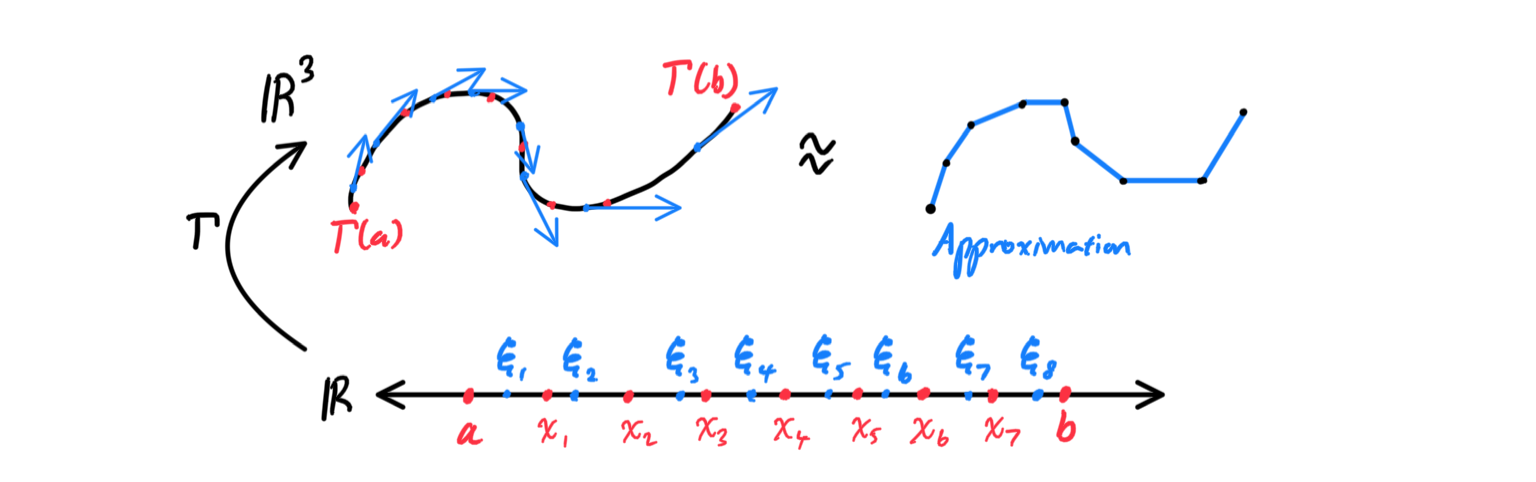
\includegraphics[scale=0.25]{img/Arc_Length_Integral.PNG}
    \caption{We can visualize this by partitioning the interval $[a, b]$ into the intervals $\Delta_i$, each with point $\xi_i \in \Delta_i$. This would partition the path to $\Gamma(\Delta_i)$, each with points $\Gamma(\xi_i)$, and at each point $\Gamma(\xi_i)$, we can imagine the velocity vector of the curve. By taking the magnitude of this vector $\Gamma^\prime (\xi_i)$, we multiply it by the length of the interval $\Delta x_i$ to get one rectangle, creating an approximation for one partition of the path. } 
    \label{fig:Arc_Length_Integral}
  \end{figure}

  \begin{corollary}[Length of the Graph of a $C^1$ Function]
    An immediate result of this formula is the formula for the length of a graph of a function $f: [a, b] \longrightarrow \mathbb{R}$ in $\mathbb{R}^2$, by looking at the paramaterization $t \mapsto (t, f(t)$. 
    \begin{equation}
      \Lambda(\gamma) = \int_a^b \sqrt{1 + (f^\prime (t))^2}\,dt
    \end{equation}
  \end{corollary}

  The question on the effect of paramaterization on the integral now arises. 

  \begin{definition}[Admissible Change of Parameter]
    The path $\Tilde{\Gamma}: [\alpha, \beta] \longrightarrow \mathbb{R}^3$ is obtained from $\Gamma: [a, b] \longrightarrow \mathbb{R}^3$ by an \textbf{admissible change of parameter} if there exists a smooth mapping 
    \[T: [\alpha, \beta] \longrightarrow [a, b]\]
    such that $T(\alpha) = a, T(\beta) = b$, $T^\prime (\tau) > 0$ (that is, the reparamaterization $T$ is monotonic) on $[\alpha, \beta]$, and 
    \[\Tilde{\Gamma} = \Gamma \circ T\]
    The series of mappings can be represented with the following commutative diagram, where $I_{\alpha, \beta} = [\alpha, \beta] \subset \mathbb{R}$ and $I_{a, b} = [a, b] \subset \mathbb{R}$. 
    \[
      \begin{tikzcd}
        I_{\alpha, \beta} \arrow{r}{T} \arrow{rd}{\Tilde{\Gamma}}& I_{a, b} \arrow{d}{\Gamma}\\
         & \mathbb{R}^3
      \end{tikzcd}
    \]

    \begin{figure}[H]
      \centering 
      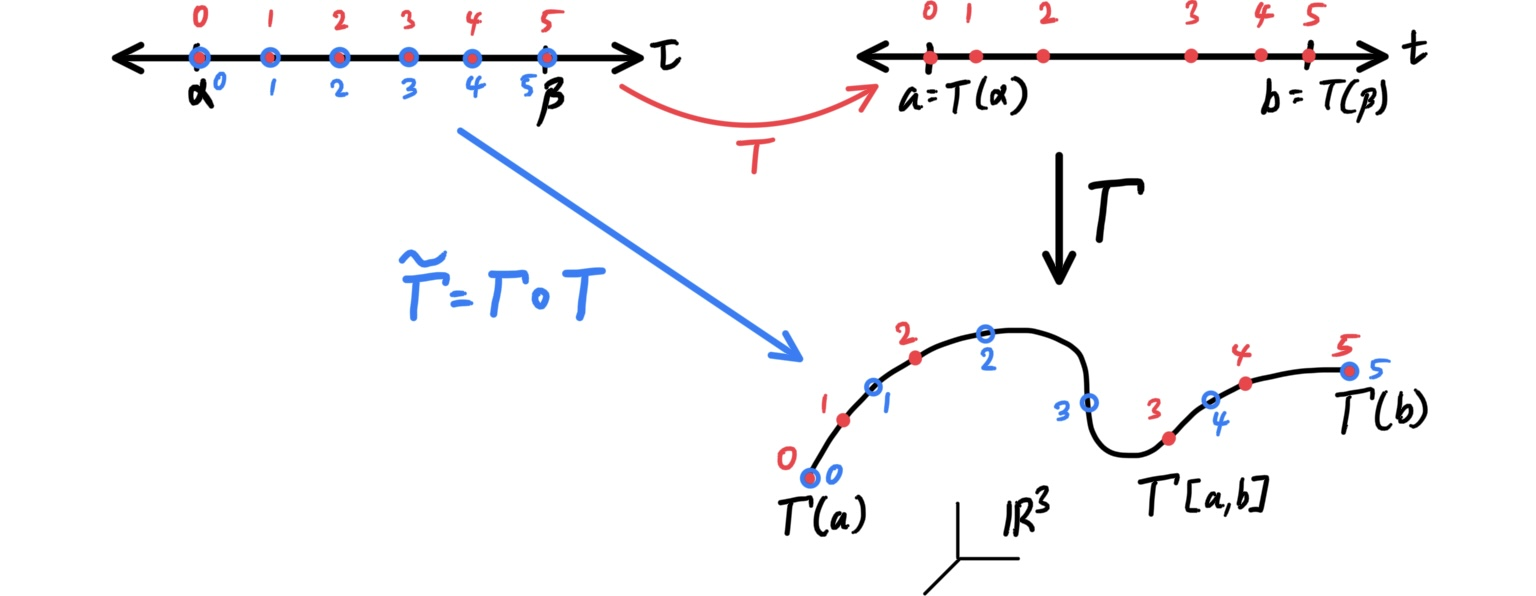
\includegraphics[scale=0.25]{img/Admissible_Change_of_Parameter.jpg}
      \caption{Note that the points are labeled $0, 1, 2, 3, 4, 5$ do not represent numerical values, but rather the order in which the points are paramaterized. We can see from this ordering that $T$ is monotonic. } 
      \label{fig:Admissible_Change_of_Parameter}
    \end{figure}
  \end{definition}

  \begin{theorem}[Invariance of Arclength Integral under Admissible Change of Parameters]
    If a smooth path $\Tilde{\Gamma}: [\alpha, \beta] \longrightarrow \mathbb{R}^3$ is obtained from a smooth path $\Gamma: [a, b] \longrightarrow \mathbb{R}^3$ by an admissible change of parameter, then the lengths of the two paths are equal. That is, a
    \begin{equation}
      \int_a^b |\Gamma^\prime (t) |\,dt = \int_\alpha^\beta |\Tilde{\Gamma}^\prime (t)|\,dt \equiv \int_\alpha^\beta |(\Gamma \circ T)^\prime (t)|\,dt
    \end{equation}
  \end{theorem}

\subsection{Improper Integrals}

  Due to some limitations of the Riemann integral, we cannot integrate over "singularities" where either the interval or the function is unbounded. We develop the tools of improper integration to deal with this problem; there are two types of improper integrals. 

  \begin{definition}[Improper Integral of Unbounded Interval]
    Suppose the function $x \mapsto f(x)$ is defined on the interval $[a, +\infty)$ and is integrable on every closed interval $[a, b]$ contained in that interval. Then, we call the following term
    \[\int_a^{+\infty} f(x)\,dx \equiv \lim_{b \rightarrow + \infty} \int_a^b f(x)\,dx\]
    the \textbf{improper Riemann integral of $f$ over the interval $[a, +\infty)$} and 
    \[\int_{-\infty}^b f(x)\,dx \equiv \lim_{a \rightarrow -\infty} \int_a^b f(x)\,dx \]
    the \textbf{improper Riemann integral of $f$ over the interval $(-\infty, b]$}.If the limit exists, then we say that the integral \textbf{converges} and \textbf{diverges} otherwise. 
  \end{definition}

  \begin{definition}[Improper Integral of Unbounded Function]
    Suppose the function $x \mapsto f(x)$ is defined on the interval $[a, B)$ and integrable on any closed interval $[a, b] \subset [a, B)$. Then, we call the following term
    \[\int_a^B f(x)\,dx \equiv \lim_{b \rightarrow B^-} \int_a^b f(x)\,dx\]
    the \textbf{improper Riemann integral of $f$ over interval $[a, B)$} and
    \[\int_A^b f(x)\,dx \equiv \lim_{a \rightarrow A^+} \int_a^b f(x)\,dx\]
    the \textbf{improper Riemann integral of $f$ over interval $(A,b]$}.
  \end{definition}

  For cohesiveness, we can combine these two definitions of improper integrals into the following one. 

  \begin{definition}[Improper Integrals]
    Let $[a, \omega)$ be a finite or infinite interval and $x \mapsto f(x)$ a function defined on that interval and integrable over every closed interval $[a, b] \subset [a, \omega)$. Then, by definition
    \[\int_a^\omega f(x)\,dx \equiv \lim_{b \rightarrow \omega} \int_a^b f(x)\,dx\]
    if this limit exists as $b \rightarrow \omega, b \in [a, \omega)$. Similarly, given the finite or infinite interval $(\omega, b]$ with $f$ integrable over every closed interval $[a, b] \subset (\omega, b]$, we have
    \[\int_\omega^b f(x)\,dx \equiv \lim_{a \rightarrow \omega} \int_a^b f(x)\,dx\]
    Note that if $\omega \in \mathbb{R}$ and $f \in \mathcal{R}[a, \omega]$, the improper integral is equivalent to the regular Riemann integral. 
    \[\int_a^\omega f(x) = \lim_{b\rightarrow \omega} \int_a^b f(x)\,dx\]
  \end{definition}

  \begin{lemma}[Properties of the Improper Integral]
    Suppose $f, g$ are functions defined on interval $[a, \omega)$ (without loss of generality, we let $\omega$ be the upper limit of integration) and integrable on every closed interval $[a, b] \subset [a, \omega)$. Suppose the improper integrals 
    \[\int_a^\omega f(x)\,dx \text{ and } \int_a^\omega g(x)\,dx\]
    are well-defined. 
    \begin{enumerate}
      \item For any $\lambda_1, \lambda_2 \in \mathbb{R}$ the function $(\lambda_1 f + \lambda_2 g)(x)$ is integrable in the improper sense on $[a, \omega)$ and
      \[\int_a^\omega (\lambda_1 f + \lambda_2 g)(x)\,dx = \lambda_1 \int_a^\omega f(x)\,dx + \lambda_2 \int_a^\omega g(x)\,dx\]
      \item For any $c \in [a, \omega)$, 
      \[\int_a^\omega f(x)\,dx = \int_a^c f(x)\,dx + \int_c^\omega f(x)\,dx\]
      \item If $\varphi: [\alpha, \gamma) \longrightarrow [a, \omega)$ is a smooth strictly monotonic mapping with $\varphi(\alpha) = a$ and $\varphi(\beta) \rightarrow \omega$ as $\beta \rightarrow \gamma^-$, then the improper integral of the function $t \mapsto (f \circ \varphi)(t) \varphi^\prime (t)$ over $[\alpha, \gamma)$ exists and 
      \[\int_a^\omega f(x)\,dx = \int_\alpha^\gamma (f \circ \varphi)(t) \varphi^\prime (t)\,dt\]
    \end{enumerate}
  \end{lemma}

  Convergence of an Improper Integral

  Note that by definition, an improper integral 
  \[\int_a^\omega f(x)\,dx \equiv \lim_{b \rightarrow \omega} \int_a^b f(x) \,dx\]
  is a limit of the function 
  \[\mathcal{F}(b) \equiv \int_a^b f(x)\,dx\]
  as $b \rightarrow \omega$. This means that we can use the Cauchy criterion to determine the convergence of this limit, and hence, existence of this improper integral. 

  \begin{theorem}[Cauchy Criterion for Convergence of an Improper Integral]
  If the function $x \mapsto f(x)$ is defined on the interval $[a, \omega)$ and integrable on every closed interval $[a, b] \subset [a, \omega)$, then the integral 
  \[\int_a^\omega f(x)\,dx\]
  converges if and only if for every $\epsilon > 0$ there exists $B \in [a, \omega)$ such that the relation
  \[\Bigg| \int_{b_1}^{b_2} f(x)\,dx \bigg| < \epsilon\]
  holds for any $b_1, b_2 \in [a, \omega)$ satisfying $B < b_1$ and $B < b_2$. 
  \end{theorem}
  \begin{proof}
  We have
  \[\int_{b_1}^{b_2} f(x)\,dx = \int_a^{b_2} f(x)\,dx - \int_a^{b_1} f(x)\,dx = \mathcal{F}(b_2) - \mathcal{F}(b_1)\]
  and therefore the condition is simply the Cauchy criterion for the existence of a limit for the function $\mathcal{F}(b)$ as $b \rightarrow \omega$. 
  \end{proof}

  \begin{definition}[Absolute Convergence of an Improper Integral]
    The improper integral 
    \[\int_a^\omega f(x)\,dx\]
    \textbf{converges absolutely} if the integral
    \[\int_a^\omega |f|(x)\,dx\]
    converges. Clearly, the inequality
    \[\Bigg| \int_{b_1}^{b_2} f(x)\,dx \Bigg| \leq \Bigg| \int_{b_1}^{b_2} |f|(x)\,dx \Bigg|\]
    implies that if an improper integral converges absolutely, then it converges. 
  \end{definition}

  This study of absolute convergence reduces to the study of convergence of integrals of nonnegative functions. The following lemma is useful in determining convergence of such functions. 

  \begin{lemma}
    Let there be a function $f$ defined on interval $[a, \omega)$ that is also integrable over every closed interval $[a, b] \subset [a, \omega)$. If $f(x) \geq 0$ on $[a, \omega)$, then the improper integral 
    \[\int_a^\omega f(x)\,dx\]
    exists if and only if the function 
    \[\mathcal{F}(b) \equiv \int_a^b f(x)\,dx\]
    is bounded on $[a, \omega)$. 
  \end{lemma}
  \begin{proof}
  It is clear that 
  \[\int_a^\omega f(x)\,dx = \lim_{b \rightarrow \omega} \mathcal{F}(b)\]
  If $f(x)\geq 0$, then the function $\mathcal{F}(b)$ is nondecreasing on $[a, \omega)$ and therefore has a limit as $b \rightarrow \omega$ only if it is bounded (since every monotonically increasing sequence that is bounded always converges). 
  \end{proof}

  This leads to the familiar integral test for convergence of a series. 

  \begin{theorem}[Integral Test for Convergence of a Series]
  If the function $x \mapsto f(x)$ is defined on the interval $[1, +\infty)$, nonnegative, nonincreasing, and integrable on each closed interval $[1, b] \subset [1, +\infty)$, then the series 
  \[\sum_{n=1}^\infty f(n) = f(1) + f(2) + \ldots\]
  and the integral 
  \[\int_a^{+\infty} f(x)\,dx\]
  either both converge or both diverge. 
  \end{theorem}

  We can use the comparison test analogue to determine convergence of improper integrals. 

  \begin{theorem}[Comparison Test for Convergence of Improper Integrals]
  Suppose the functions $f(x), g(x)$ are defined on the interval $[a, \omega)$ and integrable on any closed interval $[a, b] \subset [a, \omega)$. If 
  \[0 \leq f(x) \leq g(x)\]
  on $[a, \omega)$, then 
  \[\int_a^\omega g(x)\,dx \text{ converges} \implies \int_a^\omega f(x)\,dx \text{ converges}\]
  and the inequality 
  \[\int_a^\omega f(x)\,dx \leq \int_a^\omega g(x)\,dx\]
  holds. Also, 
  \[\int_a^\omega f(x)\,dx \text{ diverges} \implies \int_a^\omega g(x)\,dx \text{ diverges}\]
  \end{theorem}

  Improper Integrals with Multiple Singularities

  \begin{definition}[Improper Integral with Both Limits as Singularities]
    Given singularities $\omega_1, \omega_2$, the improper integral is defined
    \[\int_{\omega_1}^{\omega_2} f(x)\,dx \equiv \int_{\omega_1}^c f(x)\,dx + \int_c^{\omega_2} f(x)\,dx\]
    where $c$ is an arbitrary point in $(\omega_1, \omega_2)$. 
  \end{definition}

  \begin{example}[Gaussian Integral]
  The integral 
  \[\int_{-\infty}^{+\infty} e^{-x^2}\,dx = \sqrt{\pi}\]
  \end{example}

